\begin{appendices}
\section{More on why using Go and Python}
Companies usually try to enforce homogeneous codebases, in other words: using a single language or the minimum possible number of languages, to both make it easier to maintain the codebase and to make it easier to hire engineers.

However, in this work we have decided to use 2 languages, the reason for that is that we believe we should use the right tools for a given job.

Machine learning tooling in Python is complete and backed by a strong community, the fact that Python is a dynamically typed languages makes total difference when performing data science experiments; we usually need to add and remove features as quickly as possible, and this can become very time demanding in a statically typed language with strict policies.

On the other hand, distributed and concurrent programming in Golang is as natural as the language itself can be; after all, these programming constructs are embedded in the language. Enforcing reliability in a system built in Golang is significantly easier than in systems built in Python.

And since \projectname{} needs to provide reliability, speed, and a fast way to experiment with machine learning using an arbitrary dataset, using Python for machine learning and wrapping its service and provide a solid infrastructure using Golang was the way to go.

The communication between these two components could be done using many common strategies such as exposing the machine learning service as a REST API, or using gRPC. However, that would introduce unnecessary complexities such as an HTTP and/or TCP layer, where all the communication between them is going to happen in the same machine---at least for now. Thus, exposing the machine learning component through a clean CLI-like API, and controlling it in Golang using Bash is the easiest and fastest way to achieve this communication.

% TODO: create image graph to illustrate this

\section{More on the Finch architecture}

\subsection{The MAPE loop}
The main component in \projectname{} is the MAPE (Monitor, Analyze, Predict, and Execute) loop, this is what we are injecting into the target system, and this loop is composed of 2 inner loops: one responsible for periodically building the dataset containing the system's context, and another loop responsible for monitoring the current state of the system and triggering and carrying out adaptation plans.

These loops---1 main loop, and 2 inner loops---are implemented using Goroutines and Go's channels, which are pipes that connect concurrent goroutines. The philosophy behind Go's channel is: share by communicating, not by sharing, thus, instead of sharing memory between threads, the sharing happens by sending messages between channels.
Instead of handling concurrency by using mutex locks, it's favored by Go's community to use channels and messaging. This idea come from Hoare's Communicating Sequential Processes, or CSP (refer original paper).
This turned out to be helpful when implementing something highly concurrent as the MAPE loop.

The main loop spawns two other goroutines and control them with two different channels, as shown below

\begin{lstlisting}
func (f *Finch) StartMAPELoop() {
	ticker := time.NewTicker(MonitorFrequency * time.Second)
	quitWatcher := make(chan struct{})
	
	go f.MonitorAndAnalyzeContext(ticker, quitWatcher)
	
	datasetTicker := time.NewTicker(DatasetBuilderFrequency * time.Minute)
	datasetQuit := make(chan struct{})

	go f.buildDatasetPeriodically(datasetTicker, datasetQuit)
}
\end{lstlisting}

The goroutine that periodically builds the dataset starts an inner loop that extract all metrics from Prometheus and builds the necessary dataset for training every $DatasetBuilderFrequency$ minutes as shown below.

\lstset{aboveskip=80pt,belowskip=20pt}
\begin{lstlisting}

func buildDatasetPeriodically(tickerBuilder time.Ticker, quitBuilder chan) {
	for {
		select {
		case <-tickerBuilder.C:
			f.DatasetBuilder(true, <dataset_range>)
		case <-quitBuilder:
			ticker.Stop()
			return
		}
	}
}
\end{lstlisting}

Monitoring and analyzing the current context and state of the target system requires more non-straightforward work, such as periodically: extracting, from Prometheus, a single row of metrics of that given timestamp, analyzing, extracting, and saving the current state of all SLAs defined by the user for the target system against the current context, checking if there is any SLA violation, triggering the adaptation procedure, waiting for the adaptation to fully propagate, and checking for improvements in order to prevent unnecessary new adaptations.

\lstset{aboveskip=20pt,belowskip=20pt}
\begin{lstlisting}
	func (f *Finch) MonitorAndAnalyzeContext(ticker time.Ticker, quitWatcher chan) {
		SLAMetricsHistory := make(map[SLA][]float64)
		adaptationWasCarried := false
		isImproving := false
		for {
			select {
			case <-ticker.C:
				currentSLAMetrics := f.getSLAMetrics()
				SLAMetricsHistory = f.appendSLAMetricsHistory(SLAMetricsHistory, currentSLAMetrics)

				if f.checkForViolation(currentSLAMetrics) {

					if adaptationWasCarried {
						isImproving = f.checkForImprovement(SLAMetricsHistory)
						if !isImproving {
							adaptationWasCarried = false
						}
					}

					if !adaptationWasCarried {
						predictedOptimalKnobs := f.predictOptimalKnobs()

						f.carryAdaptationPlan(predictedOptimalKnobs)

						adaptationWasCarried = true
					}
				}
			case <-quitWatcher:
				ticker.Stop()
				return
			}
		}
	}
\end{lstlisting}


\subsection{Preventing unnecessary adaptations}
In order to prevent \projectname{} to create and carry out adaptation plans right after a previous adaptation plan was carried out, it needs to know that a previous plan has been carried out \emph{and} if there's any improvement in the target system. To know if there's any improvement is to understand and take in consideration the propagation effect of the execution of an adaptation plan, in other words: before trying, again, to predict a better configuration, it is better to wait for a previous adaptation to take full effect. The next subsection goes into more detail on how this is done.

\subsubsection{Detecting improvement after carrying out an adaptation}

We devised an algorithm in \projectname{} to detect if the target system is correctly adapting and improving, i.e: making progress. This algorithm came as an answer to the question: \emph{how do we know, given an array of historical APDEX values for the extracted SLAs, whether the target system is improving or not?}

A visual explanation to this problem is the detection of a positive slope in a graph after the adaptation was carried out as shown in the figure \ref{fig:finch3}. Upon detection of improvement (positive slope/progress), no adaptation procedure should be executed. 

The procedure we created to detect progress is a sum of the successive sums of the APDEX scores in the array containing the past $n$ historical (and current) APDEX values. For instance, using the data in the figure \ref{fig:finch3}, we have an array containing the APDEX scores (in percentage):
\[
APDEXHistoricalValues = 
  \begin{pmatrix}100 & 90 & 80 & 70 & 60 & 50 & 60 & 80 & 85 & 95 & 100\end{pmatrix}
\]

We then perform successive sums: for each $index$ in the array $APDEXHistoricalValues$, except for the last index, we get the result of the sum of:

$$
APDEXHistoricalValues[index] + APDEXHistoricalValues[index + 1]
$$

Thus, we get the array:

\[
SuccessiveSums = 
  \begin{pmatrix}-10 & -10 & -10 & -10 & -10 & 10 & 20 & 5 & 10 & 5\end{pmatrix}
\]

then, we sum the values in this $SuccessiveSums$ array, if it yields a number greater than zero, it means that the target system is improving, and we return it as a boolean value to prevent firing overlapping adaptation plans. However, we keep checking for improvements, in cases where it had an initial improvement, but for instance, the workload pattern changed, causing the the sum of the $SuccessiveSums$ to be negative, we can return a boolean as false, causing the adaptation procedure to run again.

The number $n$ of past historical values, including the current one, shown to be working well for $n=5$, meaning that we get the current APDEX score, plus other 4 that were recently extracted.

\begin{figure*}[t]
  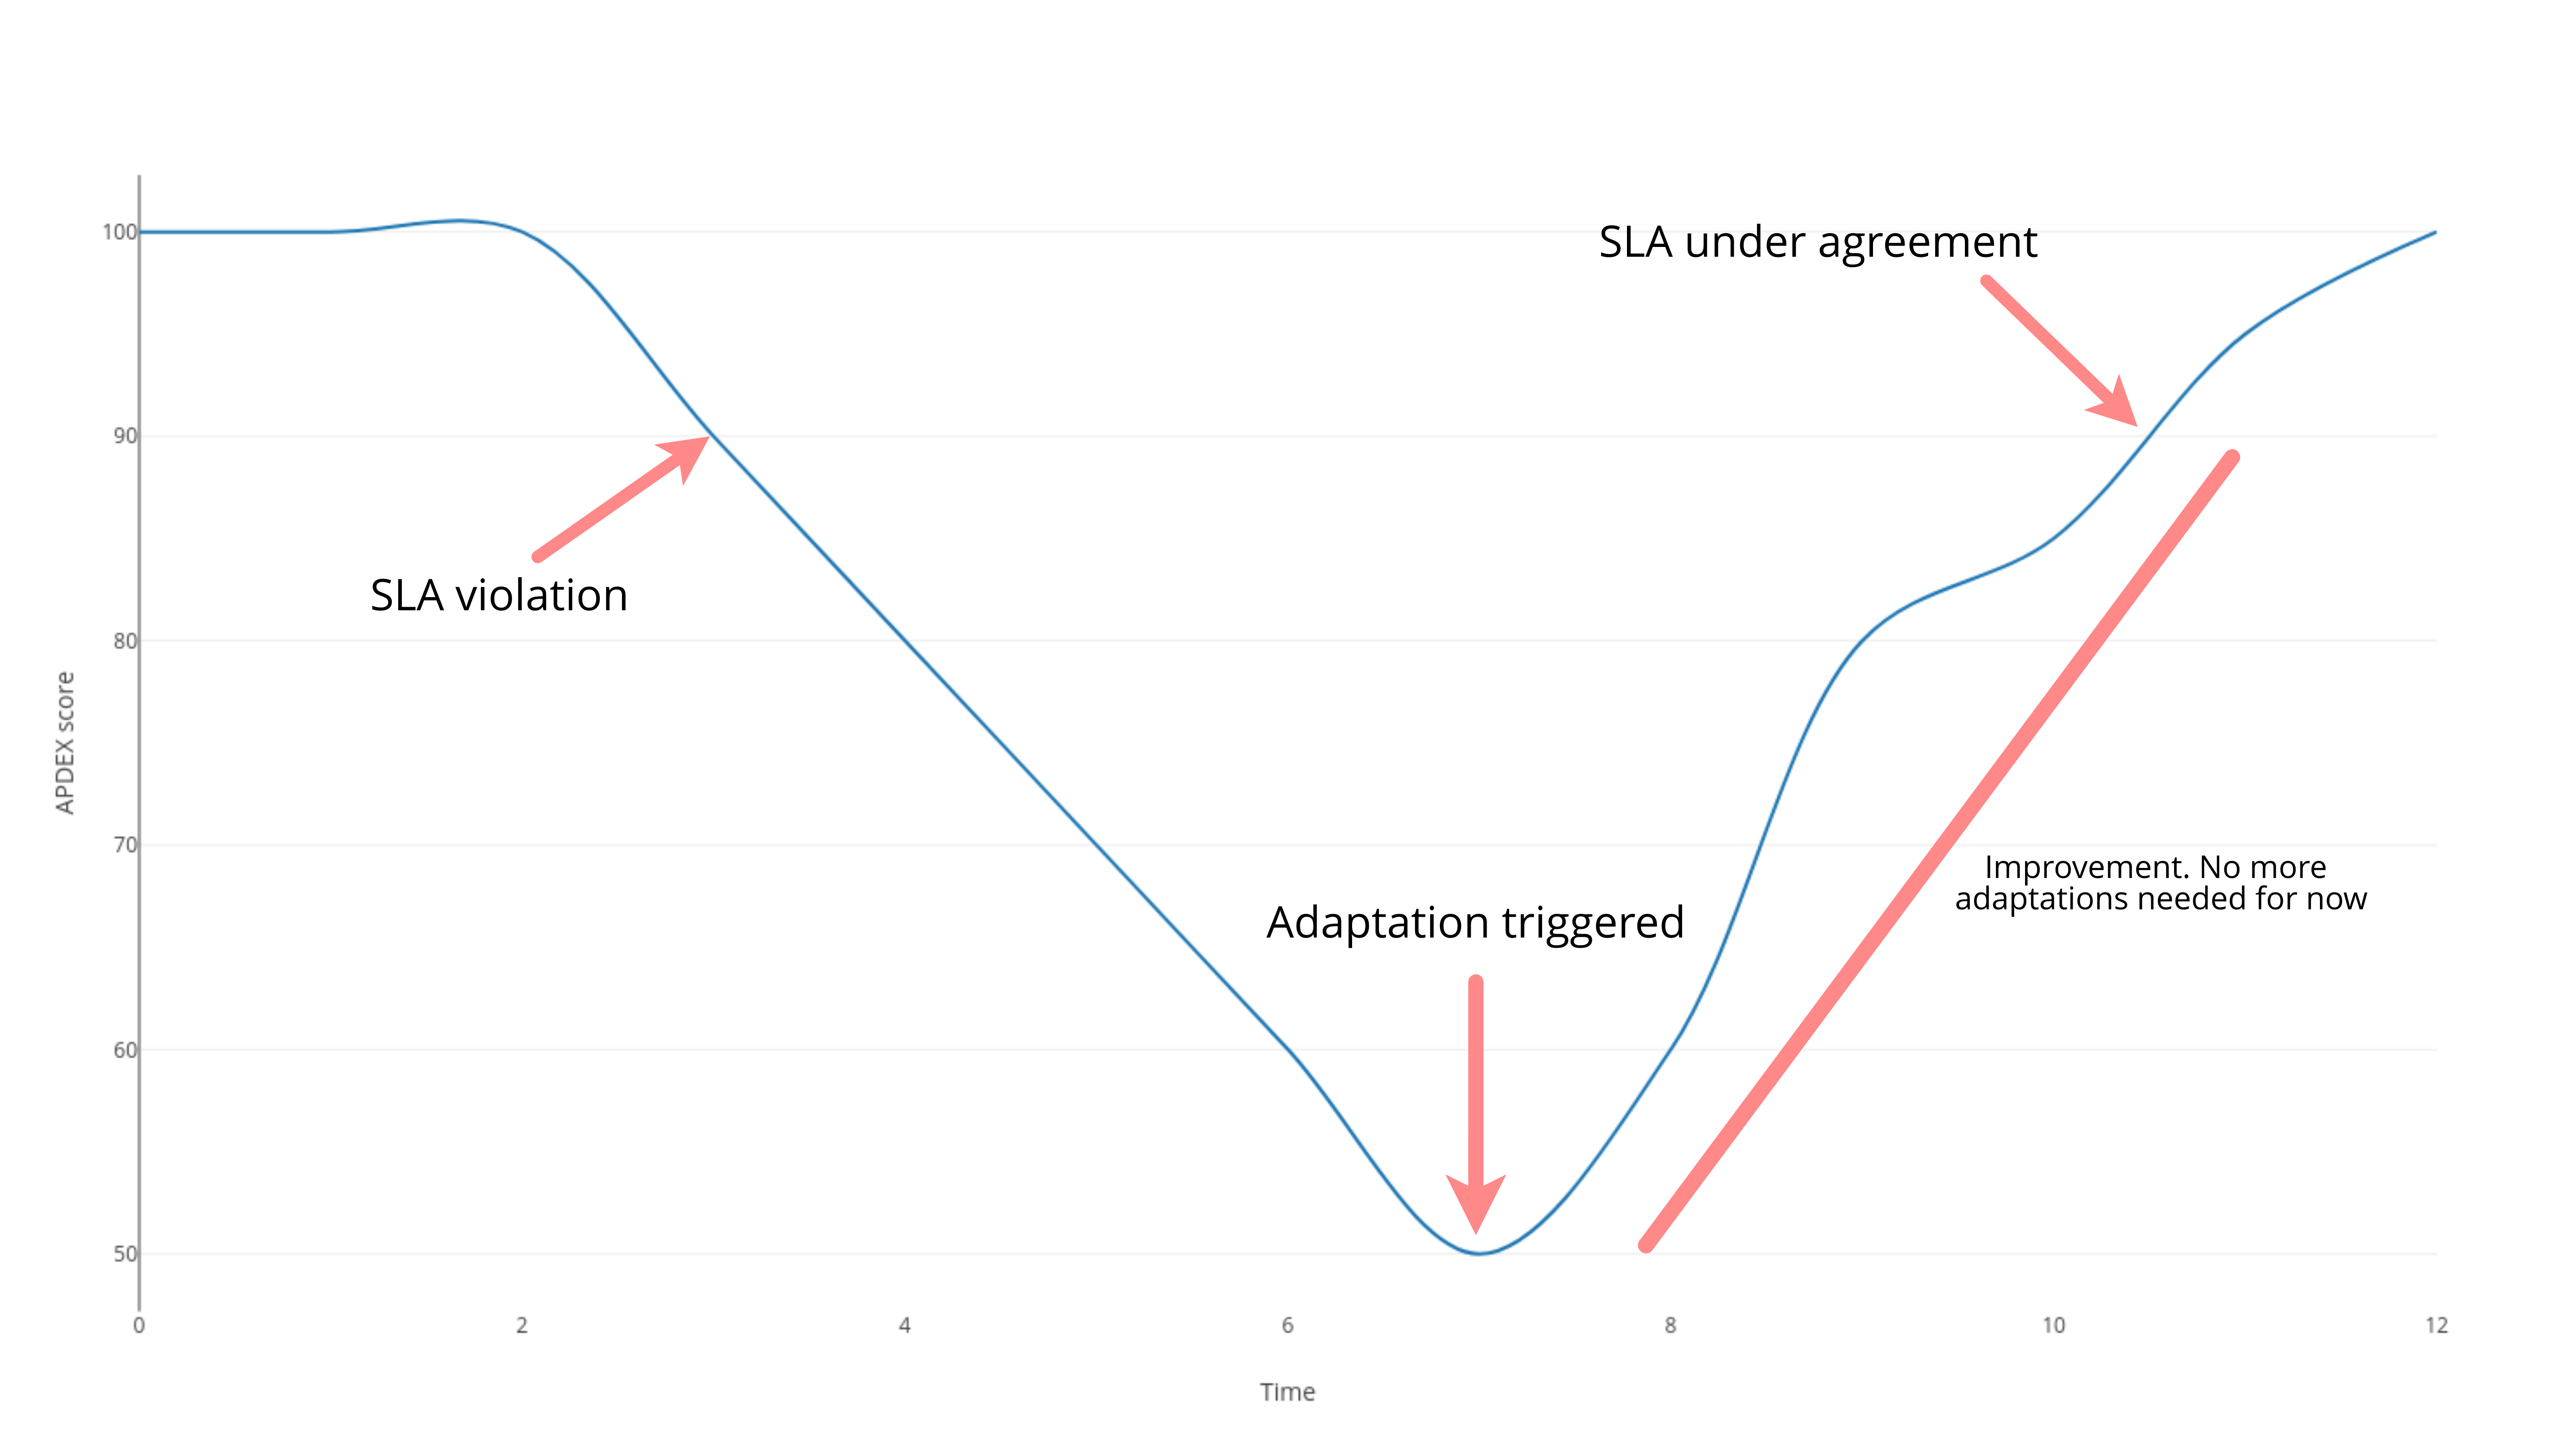
\includegraphics[scale=0.3]{images/detectImprovement.png}
  \caption{Slope that shows improvement in the target system}
  \label{fig:finch3}
\end{figure*}
\end{appendices}

\subsection{Finch configuration}

\subsubsection{Mutating configuration for initial learning}

Before the first training cycle, \projectname{} randomly changes the configurations---given a value range or possible selections---in the target system in order to learn how it behaves.


\subsubsection{SLI adjustment effect}

The experiments ran have shown an important insight: time to collect the dataset is the most crucial part of \projectname{} workflow. One of the reasons is that, in a short period of time, only the tasks that happened more frequently will have more predominance in the dataset, and thus, only configuration closely related to these tasks will have accurate predictions. Allowing the dataset to grow bigger and more diverse showed to be a good way to prevent this sort of bias.

Another reason, and an even more important one, is what we called \emph{SLI adjusment effect}. Currently, our service-level indicator for a single service is its 99th percentile of the requests latency. One important characteristics of the 99th percentile is: since it focuses on a very small sample of the data that went above the threshold and violated an SLA, it takes time for the newly adapted configuration, \emph{now actually showing signs of improvements}, to take effect on the service-level indicator. If we prematurely take this dataset, it will indicate as if the new (and correct) configuration is not a good configuration, as the 99th percentile is still violating the agreement, however, the longer we wait for the SLI to adjust to the new configuration, the better the SLI will reflect it, balancing the dataset and enabling the machine learning component to make more accurate predictions.

Simple term: the sli points don't reflect any current improvement now, it will only show improvements after a certain time.

\subsubsection{How much data is enough for good predictions?}

This is one of the most polemic questions in the machine learning community. And just like in software engineering, the answer will always be: it depends. It depends on the quality of the dataset, how many features (SLIs) are being extracted, for how long it's been collecting data, and how \projectname{} was configured to collect the data. (More on this)
